\documentclass[envcountsect]{beamer}

\usepackage[utf8]{inputenc}
\usepackage{amsmath,amsfonts,amsthm, amssymb, mathrsfs, yfonts} % Math packages
\usepackage{cancel}

\setbeamertemplate{theorems}[ams style]
\setbeamertemplate{footline}[frame number]

\usepackage{pgf, tikz}
\usetikzlibrary{arrows, automata}

\newcommand{\FF}{\mathbb{F}}
\newcommand{\A}{\mathcal{A}}
\newcommand{\C}{\mathcal{C}}
\newcommand{\R}{\mathcal{R}}
\newcommand{\card}[1]{\left\vert {#1} \right\vert}
\newcommand{\cl}{\text{Cl}}


\newtheorem{thm}{Theorem}[section]
\newtheorem{pf}{Proof}[thm]
\newtheorem{rmk}[thm]{Remark}
\newtheorem{defn}[thm]{Definition}
\newtheorem{lema}[thm]{Lemma}


\usetheme{Copenhagen}
\title{Bounds on parameters of LRC-t codes}
\author{Petar Hlad Colic}
\institute{Universitat Polit\`ecnica de Catalunya}
\date{May 2018}

\begin{document}
    \frame{\titlepage}
    
    \frame{\tableofcontents}
    
    \section{Preliminaries on LRC codes}

\begin{frame}{Notation}
    \begin{itemize}

	    \item $\C$ denotes a code over the finite field $\FF_q$.
	    
	    \item The triple of parameters $(n,k,r)$ refers to a code of:
	    \begin{itemize}
	        \item length $n$
	        \item cardinality $q^k$
	        \item locality $r$
	    \end{itemize}
	    
	    \item $[n] := \{ 1, \dots , n\}$
	    
	    \item A \textit{restriction} $\C_I$ of the code $\C$ to a subset of coordinates $I \subset [n]$ is the code obtained by removing from each vector the coordinates outside $I$.
    \end{itemize}
\end{frame}

\subsection{Definition and properties of LRC}

\begin{frame}{Definition of LRC Codes}
    Given $a \in \FF_q$ consider the sets of codewords of $\C$ with fixed value $a$ at the symbol $x_i$:

    $$ \C (i,a) = \{ x \in \C : x_i = a \}, \quad i \in [n] $$
    
    \begin{defn}
        A code $\C$ of length $n$ has \textbf{locality r} if $\ \forall i \in [n ] $ there exists a subset $I_i \subset [n] \setminus i, \quad \vert I_i \vert \leq r$ such that the restrictions of the sets $\C (i,a)$ to the coordinates in $I_i$ for different $a$ are disjoint:
        $$\C_{I_i} (i,a) \cap \C_{I_i} (i,a') = \emptyset, \quad a \neq a'.$$
    \end{defn}    
\end{frame}

\note{
Given $x \in \C$, $i \in [n]$, there exists a subset $I_i \subset [n] \setminus i$ of at most $r$ coordinates such that the restriction of $\C$ to $I_i$ enables to find the value of $x_i$.
    $I_i$ is called a \textbf{recovering set} for the symbol $x_i$.
    }
    
\begin{frame}{Bounds on rate and min. distance}
	Let $\C$ be an $(n,k,r)$ LRC code of cardinality $q^k$ over an alphabet of size $q$. Then:
    \begin{thm}[Upper bound on the rate]
        The rate of $\C$ satisfies
        $$ \frac{k}{n} \leq \frac{r}{r+1} $$
    \end{thm}
    
    \begin{thm}[Generalization of Singleton bound]
        The minimum distance of $\C$ satisfies
            $$d \leq n - k - \left\lceil \frac{k}{r} \right\rceil + 2$$
        A code that achieves the bound with equality will be called an \textbf{optimal LRC code}.
    \end{thm}
\end{frame}
    
    \begin{frame}
        \frametitle{Construction of LRC codes}
        We want to construct a linear $(n,k,r)$-LRC code. Assume $r \vert k$ and $(r+1) \vert n$.
        
        We need:
        
        \begin{itemize}
            \item $A_1 , \dots , A_{\frac{n}{r+1}}$ disjoint subsets of the field $\FF_q$, s.t. $\vert A_i \vert = r+1$
            \item $g(x) \in \FF_q[x]$ a polynomial s.t.
            \begin{enumerate}
                \item $deg(g) = r+1$
                \item $g$ is constant on each set $A_i$: $g(\alpha) = g(\beta)$ for $\alpha, \beta \in A_i$
            \end{enumerate}
        \end{itemize}                
        We will call $g$ a good polynomial.
        
    \end{frame}
    
    \begin{frame}{Construction of LRC codes}
        Let $A= \bigcup_{i=1}^{\frac{n}{r+1}} A_i \subset \FF_q$, $\vert A \vert = n$.
        
        We write now message vectors $a \in \FF_q^k$ as $r \times \frac{k}{r}$ matrices.
        
        $$ a = \;
        \begin{pmatrix}
            a_{0,0} & a_{0,1} & \cdots & a_{0,\frac{k}{r}-1} \\
            a_{1,0} & a_{1,1} & \cdots & a_{1,\frac{k}{r}-1} \\
            \vdots  & \vdots  & \ddots & \vdots \\
            a_{r-1,0} & a_{r-1,1} & \cdots & a_{r-1,\frac{k}{r}-1}
        \end{pmatrix}
        $$
    \end{frame}
    
    \begin{frame}{Construction of LRC codes}
        \begin{block}{Encoding polynomial}
            Given the message vector $a \in \FF_q^k$, define the \textbf{encoding polynomial} as:
            $$ f_a(x) = \sum_{i=0}^{r-1} x^i \cdot f_i(x) $$
            where
            $$f_i(x) = \sum_{j=0}^{\frac{k}{r}-1} a_{ij} g(x)^j $$
        \end{block}
    \end{frame}
    \begin{frame}
        $$ f_a(x) =
        \begin{pmatrix}
            x^0 & \dots & x^{r-1}
        \end{pmatrix}
        \begin{pmatrix}
            a_{0,0} & \cdots & a_{0,\frac{k}{r}-1} \\
            \vdots  & \ddots & \vdots \\
            a_{r-1,0} & \cdots & a_{r-1,\frac{k}{r}-1}
        \end{pmatrix}
        \begin{pmatrix}
            g(x)^0 \\
            \vdots \\
            g(x)^{\frac{k}{r}-1}
        \end{pmatrix} =
        $$
        
        $$
        =
        \begin{pmatrix}
            x^0 & \dots & x^{r-1}
        \end{pmatrix}
        \begin{pmatrix}
            f_0(x) \\
            \vdots \\
            f_{r-1}(x)
        \end{pmatrix}
        $$
    \end{frame}
    
    \begin{frame}
        The codeword for $a \in \FF_q^k$ is found as the evaluation vector of $f_a$ at all the points of $A$.
        \begin{block}{LRC code}
            The $(n,k,r)$ LRC code $\C$ is defined as the set of $n$-dimensional vectors
            $$\C = \{ (f_a(\alpha), \alpha \in A) : a \in \FF_q^k \}$$
        \end{block}
    \end{frame}
    
\begin{frame}
    \begin{rmk}
        $$x \in A_i \Rightarrow \quad g(x) \mbox{ constant}$$
        $$\Rightarrow f_\ell(x) = \sum_{j=0}^{\frac{k}{r}-1} a_{\ell j} g(x)^j \mbox{ constant in } A_i$$
        $$\Rightarrow \text{deg}(f_a(x)) = \text{deg}(\sum_{j=0}^{r-1} x^j \cdot f_j(x)) \leq r-1 \mbox{ in } A_i$$
    \end{rmk}
\end{frame}

\begin{frame}{Recovery of the erased symbol}
    Suppose erased symbol: $\alpha \in A_j$.
    
    Let $\left( c_{\beta}, \ \beta \in A_j \setminus \alpha \right)$ denote the remaining $r$ symbols of the recovering set.
    
    To find the value $c_{\alpha} = f_a(\alpha)$, find the unique polynomial $\delta(x)$ s.t.
    \begin{itemize}
        \item $\text{deg}(\delta(x)) \leq r$
        \item $\delta(\beta) = c_{\beta} \quad \forall \beta \in A_j \setminus \alpha$
    \end{itemize}
    
    This polynomial is:
    $$\delta(x) = \sum_{\beta \in A_j \setminus \alpha} c_{\beta} \prod_{\beta ' \in A_j \setminus \{\alpha, \beta\}} \frac{x - \beta'}{\beta - \beta '}$$

    Finally, set $c_{\alpha} = \delta(\alpha)$.
    
\end{frame}

\begin{frame}
    \begin{thm}
        The linear code $\C$ defined has dimension $k$ and is an optimal $(n,k,r)$ LRC code.
    \end{thm}
\end{frame}

\begin{frame}
    \begin{proof}[Proof of dimension]
        For $i \in \{0, \dots, r-1 \}$; $j \in \{0, \dots, \frac{k}{r-1}\}$ the $k$ polynomials $g(x)^j x^i$ all are of distinct degrees, i.e. linearly independent over $\FF$.
        
        $\Rightarrow$ The mapping $a \mapsto f_a$ is injective.
        
        $$\mbox{deg}(f_a(x)) \leq \mbox{deg}(x^{r-1}) + \mbox{deg}(g(x)^{\frac{k}{r}-1}) = r-1 + (r+1)(\frac{k}{r}-1)$$
        $$= k + \frac{k}{r} - 2 \leq n - 2$$
        
        This means that two distinct encoding polynomials give rise to two distinct codevectors. $\quad \Rightarrow \quad $ The dimension of the code is $k$.
    \end{proof}
\end{frame}

\begin{frame}
    \begin{proof}[Proof of optimality]
        Since the encoding is linear:
        $$d(\C) \geq n - \max_{f_a, a\in \FF_q^k} \mbox{deg}(f_a) = n - k - \frac{k}{r} + 2 \geq n - k - \left\lceil\frac{k}{r}\right\rceil + 2$$
        But we have that $d(\C) \leq n - k - \left\lceil\frac{k}{r}\right\rceil + 2$.
        Therefore, we have equality and thus it is an optimal LRC Code.
    \end{proof}
\end{frame}
    
    \begin{frame}{Example: (9,4,2) LRC code}
        We will now construct a $(n=9, k=4, r=2)$ LRC code over the field $\FF_q$.
        
        $$q = \vert \FF_q \vert \geq n \quad \Rightarrow \quad q \geq 9$$
        
        Choose $q = 13$
        
        $$\A = \{ A_1 = \{1,3,9\}, A_2 = \{2,6,5 \}, A_3 = \{4,12,10 \} \}$$.
        
        $$g(x) = x^3 = 
        \begin{cases}
            1 & \mbox{if } x \in A_1 \\
            8 & \mbox{if } x \in A_2 \\
            12& \mbox{if } x \in A_3
        \end{cases}
        $$
    \end{frame}
    
    \begin{frame}
        For $a = 
        \begin{pmatrix}
            a_{00} & a_{01} \\
            a_{10} & a_{11}
        \end{pmatrix} \in \FF_{13}^4$ define the encoding polynomial:
        $$f_a(x) =
        \begin{pmatrix}
            1 & x
        \end{pmatrix}
        \begin{pmatrix}
            a_{00} & a_{01} \\
            a_{10} & a_{11}
        \end{pmatrix}
        \begin{pmatrix}
            1 \\
            x^3
        \end{pmatrix} = a_{00} + a_{10}x + a_{01} x^3 + a_{11} x^4
        $$
        
        E.g. $a =         
        \begin{pmatrix}
            1 & 1 \\
            1 & 1
        \end{pmatrix}
        $. $f_a(x) = 1 + x + x^3 + x^4$
        
        $$c = (f_a(1), f_a(3), f_a(9), f_a(2), f_a(6), f_a(5), f_a(4), f_a(12), f_a(10))$$
        $$= (4,8,7,1,11,2,0,0,0)$$
    \end{frame}        
    
    \begin{frame}
        \onslide<1->{
        $$\delta(x) = \sum_{\beta \in A_j \setminus \alpha} c_{\beta} \prod_{\beta ' \in A_j \setminus \{\alpha, \beta\}} \frac{x - \beta'}{\beta - \beta '}$$    
    
        $$(
        \only<1,6->{f_a(1)}\only<2-5>{\textcolor{red}{\xcancel{f_a(1)}}},
        f_a(3),
        f_a(9),
        \only<1-5,10->{f_a(2)}\only<6-9>{\textcolor{red}{\xcancel{f_a(2)}}},
        f_a(6),
        f_a(5),
        \only<1-9>{f_a(4)}\only<10-13>{\textcolor{red}{\xcancel{f_a(4)}}},
        f_a(12),
        f_a(10))
        $$
        $$(
        \only<1,6->{4}\only<2-5>{\textcolor{red}{\xcancel{4}}},
        8,
        7,
        \only<1-5,10->{1}\only<6-9>{\textcolor{red}{\xcancel{1}}},
        11,
        2,
        \only<1-9>{0}\only<10-13>{\textcolor{red}{\xcancel{0}}},
        0,
        0
        )$$
        }
        \begin{overlayarea}{\textwidth}{0.3\textheight}
        \only<2-5>{
            \only<3-5>{$$ 1 \in A_1 = \{ 1, 3, 9 \}$$}
            \only<4-5>{$$ \Rightarrow \delta(x) = c_3 \frac{x-9}{3-9} + c_9 \frac{x-3}{9-3} = 2x + 2 $$}
            \only<5>{$$\delta(1) = 4$$}
        }
        
        \only<6-9>{
            \only<7-9>{$$ 2 \in A_2 = \{ 2, 6, 5 \}$$ }
            \only<8-9>{$$ \Rightarrow \delta(x) = c_6 \frac{x-5}{6-5} + c_5 \frac{x-6}{5-6} = 9x + 9$$}
            \only<9>{$$\delta(2) = 1$$}
        }
        
        \only<10-13>{
            \only<11-13>{$$4 \in A_3 = \{ 4,12,10 \}$$}
            \only<12-13>{$$ \Rightarrow \delta(x) = c_{12} \frac{x-10}{12-10} + c_{10} \frac{x-12}{10-12} = 0$$}
            \only<13>{$$\delta(4) = 0$$}
        }
        \end{overlayarea}
        
    \end{frame}
    
    \begin{frame}
        \frametitle{Example of LRC-2 code}
        
        Let $\FF = \FF_{13}$, $A = \FF \setminus \{0\}$
        
        $\mathcal{A} = \left\lbrace  \left\lbrace 1, 5, 12 , 8 \right\rbrace, \left\lbrace 2 , 10 , 11 , 3 \right\rbrace , \left\lbrace 4 , 7 , 9 , 6 \right\rbrace \right\rbrace$
        
        $\mathcal{A'} = \left\lbrace  \left\lbrace 1 , 3 , 9 \right\rbrace, \left\lbrace 2 , 6 , 5 \right\rbrace , \left\lbrace 4 , 12 , 10 \right\rbrace , \left\lbrace 7 , 8 , 11 \right\rbrace \right\rbrace$
        
        $f_a(x) = a_0 + a_1 x + a_2 x^4 + a_3 x^6$
        
        $$a = (1,1,1,1) \quad \longrightarrow \quad c = (4,8,7,5,2,6,2,2,2,3,9,1)$$
        
        As already seen: $\delta(x) = 2x + 2$; $\delta(1)=4$.
        $$\delta ' (x) = c_5 \frac{x-12}{5-12}\frac{x-8}{5-8} + c_{12} \frac{x-5}{12-5}\frac{x-8}{12-8} + c_8 \frac{x-5}{8-5}\frac{x-12}{8-12}$$
        $$ = 6 \cdot 5 \cdot (x^2 + 6x + 5) + 2 \cdot 7 \cdot (x^2 + 1) + 9 \cdot 1 \cdot (x^2 + 9x + 8)$$
        $$ = x^2 + x + 2 \quad \longrightarrow \quad \delta ' (1) = 4$$
    \end{frame}        
    
    \section{Bounds on LRC-t codes}
\subsection{Recovery graph}
\begin{frame}{Recovery graph}

        Assume every coordinate $i$ has $t$ disjoint recovering sets $\R_i^1, \dots, \R_i^t$, each of size $r$, where $\R_i^j \subset \left[n \right] \setminus i$.
        \begin{block}{Definition}
            The \textbf{recovery graph} of a $(n,k,r,t)$ LRC code $\mathcal{C}$ is a directed graph $G=(V,E)$ where:
            \begin{itemize}
                \item $V = \left[n \right]$. (Vertices $\leftrightarrow$ coordinates of $\mathcal{C}$).
                \item $(i,j) \in E \iff j \in \R_i^\ell$ for some $\ell \in \left[ t \right]$.\\
                There is an edge $i \rightarrow j$ if $j$ is in a recovering set of $i$.\\
            \end{itemize}    
                Note that $N(i) = \bigcup_{\ell = 1}^{t} \R_i^\ell$
        \end{block}
    \end{frame}    
\subsection{Statements of the bounds}
\begin{frame}
    Let $C$ be an $(n,k,r,t)$ LRC code with $t$ dijsoint recovering sets of size $r$. Then:
    \begin{thm}
        \label{thm:max_rate_t}
        The rate of $C$ satisfies
        $$ \frac{k}{n} \leq \frac{1}{\prod_{j=1}^{t} (1 + \frac{1}{jr} )} $$
    \end{thm}
    
    \begin{thm}
        \label{thm:min_dist_t}
        The minimum distance of $C$ is bounded above as follows
        $$ d \leq n - \sum_{i=0}^{t} \left\lfloor \frac{k-1}{r^i} \right\rfloor $$
    \end{thm}
\end{frame}    
    
\subsection{Definitions and examples for the proof}
    
    \begin{frame}
    Recovery graph for the $(9,4,2)$-LRC code.
    
    Recall: $\A = \{ A_1 = \{1,3,9\}, A_2 = \{2,6,5 \}, A_3 = \{4,12,10 \} \}$
        \begin{center}
        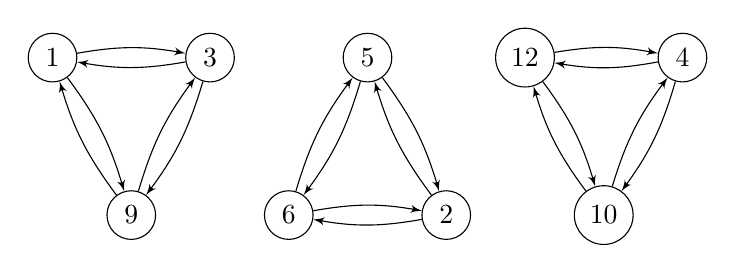
\begin{tikzpicture}
        
            \tikzset{vertex/.style = {shape=circle,draw,minimum size=1.5em}}	
            \tikzset{edge/.style = {->,> = latex'}}
            
	        \node[vertex] (n1) at (0,0) {$1$};
	        \node[vertex] (n3) at (2,0) {$3$};
	        \node[vertex] (n9) at (1,-2) {$9$};
	        
	        \node[vertex] (n6) at (3,-2) {$6$};
	        \node[vertex] (n2) at (5,-2) {$2$};
	        \node[vertex] (n5) at (4,0) {$5$};

	        \node[vertex] (n12) at (6,0) {$12$};
	        \node[vertex] (n4)  at (8,0) {$4$};
	        \node[vertex] (n10) at (7,-2) {$10$};
	        
	        \draw[edge] (n1) to [bend left=10] (n3);
	        \draw[edge] (n1) to [bend left=10] (n9);
	        \draw[edge] (n3) to [bend left=10] (n1);
	        \draw[edge] (n3) to [bend left=10] (n9);
	        \draw[edge] (n9) to [bend left=10] (n1);
	        \draw[edge] (n9) to [bend left=10] (n3);
	        
	        \draw[edge] (n2) to [bend left=10] (n5);
	        \draw[edge] (n2) to [bend left=10] (n6);
	        \draw[edge] (n5) to [bend left=10] (n2);
	        \draw[edge] (n5) to [bend left=10] (n6);
	        \draw[edge] (n6) to [bend left=10] (n2);
	        \draw[edge] (n6) to [bend left=10] (n5);
	        
	        \draw[edge] (n4) to [bend left=10] (n10);
	        \draw[edge] (n4) to [bend left=10] (n12);
	        \draw[edge] (n10) to [bend left=10] (n4);
	        \draw[edge] (n10) to [bend left=10] (n12);
	        \draw[edge] (n12) to [bend left=10] (n4);
	        \draw[edge] (n12) to [bend left=10] (n10);
	
	        %\draw[red, dashed] (1, 2) -- (1, -2);
	            
        \end{tikzpicture}
        \end{center}
    \end{frame}
    
     \begin{frame}
        Color the edges with $t$ distinct colors to differenciate recovering sets.
        
        Let $F$ be a coloring function of the edges:
        $$
            \begin{array}{ccccc}
                F: & E(G) & \longrightarrow & [t]  & \\
                   &(i,j) & \longmapsto     & \ell & \mbox{iff } j \in \R_i^\ell
            \end{array}
        $$
        
    Remark: the out-degree of any vertex $i \in V$ is $\sum_\ell \vert \R_i^\ell \vert = tr$, and the edges leaving $i$ are colored in $t$ colors.
    
    \end{frame}    
    
    \begin{frame}
    Recovery graph for the $(12,4,\{2,3\})$-LRC code with edge coloring.
    
    Recall: 
    
    $\mathcal{A} = \left\lbrace  \left\lbrace 1, 5, 12 , 8 \right\rbrace, \left\lbrace 2 , 10 , 11 , 3 \right\rbrace , \left\lbrace 4 , 7 , 9 , 6 \right\rbrace \right\rbrace$
        
     $\mathcal{A'} = \left\lbrace  \left\lbrace 1 , 3 , 9 \right\rbrace, \left\lbrace 2 , 6 , 5 \right\rbrace , \left\lbrace 4 , 12 , 10 \right\rbrace , \left\lbrace 7 , 8 , 11 \right\rbrace \right\rbrace$
     \begin{center}
        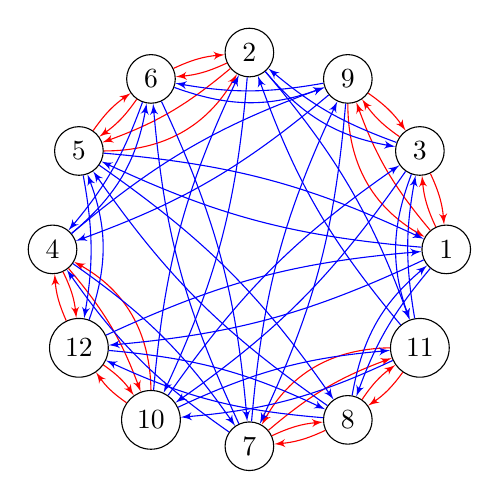
\begin{tikzpicture}
            \tikzset{vertex/.style = {shape=circle,draw,minimum size=1.5em}}	
            \tikzset{edge/.style = {->,> = latex',red}}
            \tikzset{edge2/.style = {->,> = latex',blue}}
            
            \def \radius {2.5cm}
            \def \n {12}
            
	        \node[vertex] (n1) at ({360/\n * (0)}:\radius) {$1$};
	        \node[vertex] (n3) at ({360/\n * (1)}:\radius) {$3$};
	        \node[vertex] (n9) at ({360/\n * (2)}:\radius) {$9$};
	        
	        \node[vertex] (n2) at ({360/\n * (3)}:\radius) {$2$};
	        \node[vertex] (n6) at ({360/\n * (4)}:\radius) {$6$};
	        \node[vertex] (n5) at ({360/\n * (5)}:\radius) {$5$};
	        
	        \node[vertex] (n4) at ({360/\n * (6)}:\radius) {$4$};
	        \node[vertex] (n12)  at ({360/\n * (7)}:\radius) {$12$};
	        \node[vertex] (n10) at ({360/\n * (8)}:\radius) {$10$};
	        
	        \node[vertex] (n7) at ({360/\n * (9)}:\radius) {$7$};
	        \node[vertex] (n8)  at ({360/\n * (10)}:\radius) {$8$};
	        \node[vertex] (n11) at ({360/\n * (11)}:\radius) {$11$};
	        
	        \draw[edge] (n1) to [bend left=10] (n3);
	        \draw[edge] (n1) to [bend left=10] (n9);
	        \draw[edge] (n3) to [bend left=10] (n1);
	        \draw[edge] (n3) to [bend left=10] (n9);
	        \draw[edge] (n9) to [bend right=30] (n1);
	        \draw[edge] (n9) to [bend left=10] (n3);
	        
	        \draw[edge] (n2) to [bend left=10] (n5);
	        \draw[edge] (n2) to [bend left=10] (n6);
	        \draw[edge] (n5) to [bend right=30] (n2);
	        \draw[edge] (n5) to [bend left=10] (n6);
	        \draw[edge] (n6) to [bend left=10] (n2);
	        \draw[edge] (n6) to [bend left=10] (n5);
	        
	        \draw[edge] (n4) to [bend left=10] (n10);
	        \draw[edge] (n4) to [bend left=10] (n12);
	        \draw[edge] (n10) to [bend right=30] (n4);
	        \draw[edge] (n10) to [bend left=10] (n12);
	        \draw[edge] (n12) to [bend left=10] (n4);
	        \draw[edge] (n12) to [bend left=10] (n10);
	        
	        \draw[edge] (n7) to [bend left=10] (n8);
	        \draw[edge] (n7) to [bend left=10] (n11);
	        \draw[edge] (n8) to [bend left=10] (n7);
	        \draw[edge] (n8) to [bend left=10] (n11);
	        \draw[edge] (n11) to [bend left=10] (n8);
	        \draw[edge] (n11) to [bend right=30] (n7);
	        
	        \draw[edge2] (n1) to [bend left=10] (n5);
	        \draw[edge2] (n1) to [bend left=10] (n12);
	        \draw[edge2] (n1) to [bend right=10] (n8);
	        
	        \draw[edge2] (n5) to [bend left=10] (n1);
	        \draw[edge2] (n5) to [bend left=10] (n12);
	        \draw[edge2] (n5) to [bend left=10] (n8);
	        
	        \draw[edge2] (n12) to [bend right=20] (n5);
	        \draw[edge2] (n12) to [bend left=10] (n1);
	        \draw[edge2] (n12) to [bend left=10] (n8);
	        
	        \draw[edge2] (n8) to [bend left=10] (n5);
	        \draw[edge2] (n8) to [bend left=10] (n12);
	        \draw[edge2] (n8) to [bend left=20] (n1);
	        
	        
	        \draw[edge2] (n2) to [bend right=20] (n3);
	        \draw[edge2] (n2) to [bend left=10] (n10);
	        \draw[edge2] (n2) to [bend left=10] (n11);
	        
	        \draw[edge2] (n3) to [bend left=10] (n2);
	        \draw[edge2] (n3) to [bend left=10] (n10);
	        \draw[edge2] (n3) to [bend right=20] (n11);
	        
	        \draw[edge2] (n10) to [bend left=10] (n3);
	        \draw[edge2] (n10) to [bend left=10] (n2);
	        \draw[edge2] (n10) to [bend left=10] (n11);
	        
	        \draw[edge2] (n11) to [bend left=10] (n3);
	        \draw[edge2] (n11) to [bend left=10] (n10);
	        \draw[edge2] (n11) to [bend left=10] (n2);

	        
	        \draw[edge2] (n4) to [bend right=20] (n6);
	        \draw[edge2] (n4) to [bend left=10] (n7);
	        \draw[edge2] (n4) to [bend left=10] (n9);
	        
	        \draw[edge2] (n6) to [bend left=10] (n4);
	        \draw[edge2] (n6) to [bend left=10] (n7);
	        \draw[edge2] (n6) to [bend right=20] (n9);
	        
	        \draw[edge2] (n7) to [bend left=10] (n6);
	        \draw[edge2] (n7) to [bend left=10] (n4);
	        \draw[edge2] (n7) to [bend left=10] (n9);
	        
	        \draw[edge2] (n9) to [bend left=10] (n6);
	        \draw[edge2] (n9) to [bend left=10] (n7);
	        \draw[edge2] (n9) to [bend left=10] (n4);
	            
        \end{tikzpicture}
        \end{center}
    \end{frame}
    
    
    \begin{frame}
    Recovery graph for the $(12,4,\{2,3\})$-LRC code with edge coloring.
    
    Recall: 

    $
        \mathcal{A} = \left\lbrace
        \only<5>{\textcolor{blue}}{\left\lbrace 1, 5, 12 , 8 \right\rbrace},
        \only<6>{\textcolor{blue}}{\left\lbrace 2 , 10 , 11 , 3 \right\rbrace},
        \only<7>{\textcolor{blue}}{\left\lbrace 4 , 7 , 9 , 6 \right\rbrace}
        \right\rbrace
    $
    
     $ 
         \mathcal{A'} = \left\lbrace
         \only<1>{\textcolor{red}}{\left\lbrace 1 , 3 , 9 \right\rbrace},
         \only<2>{\textcolor{red}}{\left\lbrace 2 , 6 , 5 \right\rbrace},
         \only<3>{\textcolor{red}}{\left\lbrace 4 , 12 , 10 \right\rbrace},
         \only<4>{\textcolor{red}}{\left\lbrace 7 , 8 , 11 \right\rbrace}
         \right\rbrace
     $   
        \begin{center}
        \begin{tikzpicture}
            \tikzset{vertex/.style = {shape=circle,draw,minimum size=1.5em}}	
            \tikzset{edge1/.style = {-,> = latex',red}}
            \tikzset{edge2/.style = {-,> = latex',blue}}
            
            \def \radius {2.5cm}
            \def \n {12}
            
	        \node[vertex] (n1) at ({360/\n * (0)}:\radius) {$1$};
	        \node[vertex] (n3) at ({360/\n * (1)}:\radius) {$3$};
	        \node[vertex] (n9) at ({360/\n * (2)}:\radius) {$9$};
	        
	        \node[vertex] (n2) at ({360/\n * (3)}:\radius) {$2$};
	        \node[vertex] (n6) at ({360/\n * (4)}:\radius) {$6$};
	        \node[vertex] (n5) at ({360/\n * (5)}:\radius) {$5$};
	        
	        \node[vertex] (n4) at ({360/\n * (6)}:\radius) {$4$};
	        \node[vertex] (n12)  at ({360/\n * (7)}:\radius) {$12$};
	        \node[vertex] (n10) at ({360/\n * (8)}:\radius) {$10$};
	        
	        \node[vertex] (n7) at ({360/\n * (9)}:\radius) {$7$};
	        \node[vertex] (n8)  at ({360/\n * (10)}:\radius) {$8$};
	        \node[vertex] (n11) at ({360/\n * (11)}:\radius) {$11$};
	        
	        \only<1,8>{
	        \draw[edge1] (n1) to (n3);
	        \draw[edge1] (n1) to (n9);
	        \draw[edge1] (n3) to (n9);
	        }
	        
	        \only<2,8>{
	        \draw[edge1] (n2) to (n6);
	        \draw[edge1] (n2) to (n5);
	        \draw[edge1] (n5) to (n6);
	        }
	        
	        \only<3,8>{
	        \draw[edge1] (n4) to (n10);
	        \draw[edge1] (n4) to (n12);
	        \draw[edge1] (n12) to (n10);
	        }
	        
	        \only<4,8>{
	        \draw[edge1] (n7) to (n8);
	        \draw[edge1] (n7) to (n11);
	        \draw[edge1] (n8) to (n11);
	        }
	        
	        \only<5,8>{
	        \draw[edge2] (n1) to (n5);
	        \draw[edge2] (n1) to (n12);
	        \draw[edge2] (n1) to (n8);
	        \draw[edge2] (n5) to (n12);
	        \draw[edge2] (n5) to (n8);
	        \draw[edge2] (n8) to (n12);
	        }
	        
	        \only<6,8>{
	        \draw[edge2] (n2) to (n10);
	        \draw[edge2] (n2) to (n11);
	        \draw[edge2] (n2) to (n3);
	        \draw[edge2] (n10) to (n11);
	        \draw[edge2] (n10) to (n3);
	        \draw[edge2] (n11) to (n3);
	        }
	        
	        \only<7,8>{
	        \draw[edge2] (n4) to (n7);
	        \draw[edge2] (n4) to (n9);
	        \draw[edge2] (n4) to (n6);
	        \draw[edge2] (n7) to (n9);
	        \draw[edge2] (n7) to (n6);
	        \draw[edge2] (n9) to (n6);
	        }
	        
    \end{tikzpicture}
    \end{center}
\end{frame}

\subsection{Proof for the rate bound}

\begin{frame}
    \begin{lema}
        \label{lemma:rate_lemma}
        There exists a subset of the vertices $U \subseteq V$ of size at least
        $$ \vert U \vert \geq n \left( 1 - \frac{1}{\prod_{j=1}^{t} \left(1 + \frac{1}{jr} \right)} \right) $$
        such that for any $U' \subseteq U$, $G_{U'}$ has at least one vertex $v \in U'$ such that its set of outgoing edges is missing at least one color.
    
    \end{lema}
\end{frame}

\begin{frame}
    For a given permutation $\tau$ of the set of vertices $V$, define the coloring of some of the vertices.
    
    The color $j \in [t]$ is assigned to $v$ if
    $$\tau(v) > \tau(m) \quad \forall m \in \R_v^j$$
    
    If this condition is satisfied for several values of $m$, the vertex $v$ is assigned any of these colors.
    
    If this condition is not satisfied at all, the vertex $v$ is not colored.
\end{frame}

\begin{frame}
    Let $U$ be the set of colored vertices. Consider one of its subsets $U' \subseteq U$.
    
    Assume toward a contradiction that every vertex of $G_{U'}$ has outgoing edges of all $t$ colors.
    
    Choose a vertex $v \in U'$ and construct the following walk: if the path ends at some vertex with color $j$, choose one of its outgoing edges colored in $j$.
    $$\textcolor{red}{v_1 \longrightarrow } \textcolor{blue}{v_2 \longrightarrow} \textcolor{green}{v_3 \longrightarrow} \dots \textcolor{orange}{\longrightarrow} v_\ell$$
    We can extend this path indefinitely as every vertex has outgoing edges of all $t$ colors.
\end{frame}

\begin{frame}
    Since the graph $G_{U'}$ is finite, there will be a vertex (call it $v_1$) that is encountered twice.

    $$\textcolor{red}{v_1 \longrightarrow } \textcolor{blue}{v_2 \longrightarrow} \textcolor{green}{v_3 \longrightarrow} \dots \textcolor{orange}{\longrightarrow} v_\ell \longrightarrow \textcolor{red}{v_1}$$
    
    But:
        $$
            \left .
                \begin{matrix}
                    v_i & \mbox{ color j} \\
                    (v_i, v_{i+1}) & \mbox{ color j}
                \end{matrix}
            \right \}
            \Longrightarrow \tau (v_i) > \tau (v_{i+1})
        $$
        
        $$
            \tau (v_1) > \tau (v_2) > \dots > \tau (v_\ell) > \tau (v_1) 
        $$
        
        Contradiction!!!
        
        Then, there must be a vertex in $U'$ such that its set of outgoing edges is missing one color.
        
\end{frame}

\begin{frame}
    To show that there exists such $U$ of large carinality, we choose $\tau$ uniformly at random among $\mathfrak{S}_n$ and compute $E(\card{U})$.
    
    Let $A_{v,j}$ be the event that the equation $\tau(v) > \tau(m) \quad \forall m \in \R_v^j$ holds for the vertex $v$ and the color $j$.
    Since all vertices have $r$ outgoing edges for each of the $t$ different colors, the probability $Pr(A_{v,j})$ does not depend on $v$, we write $A_{j} :=  A_{v,j}$.
    
    Recall that $v \in U$ if $v$ is colored with some color $\ell$, and is colored with $\ell$ if $A_{\ell}$ happens.
    $$Pr(v \in U) = Pr(\bigcup_{j=1}^{t} A_j)$$
\end{frame}

\begin{frame}
    Inclusion-exclusion formula: 
    $$Pr(\bigcup_{j=1}^{t} A_j) = \sum_{\emptyset \neq S \subseteq [t]} (-1)^{\card{S} - 1} Pr( \bigcap_{j\in S} A_j )$$.
    
    For that, we need, for any set $S \subseteq [t]$ the probability that all the $A_j, j \in S$ occur simultaneously.
    $$
        Pr(\bigcap_{j\in S} A_j ) = \frac{1}{\card{S}r+1}
    $$
    
    \begin{proof}
        For any assignation of values given to $\{v\} \cup ( \bigcup_{j\in S} R_v^j)$, only $1$ out of $\card{S} r + 1$ is the maximum.
    \end{proof}
\end{frame}

\begin{frame}
    $$
        Pr(\bigcup_{j=1}^{t} A_j)
        = \sum_{\emptyset \neq S \subseteq [t]} (-1)^{\card{S} - 1} Pr( \bigcap_{j\in S} A_j )
    $$
    $$
        = \sum_{\emptyset \neq S \subseteq [t]} (-1)^{\card{S} - 1} \frac{1}{\card{S}r+1}
        = \sum_{j=1}^{t} (-1)^{j - 1} \binom{t}{j} \frac{1}{\card{S}r+1}
    $$
    $$
        = 1 - \frac{1}{ \prod_{j=1}^{t} \left(1 + \frac{1}{jr} \right) }
    $$
\end{frame}

\begin{frame}
    Let $X_v$ be the indicator for the event that $v \in U$.
    
    $$
        E(\card{U})
        = \sum_{v \in V} E(X_v)
        = \sum_{v \in V} Pr(v \in U)
        = n \cdot Pr(\bigcup_{j=1}^{t} A_j)
    $$
    $$
        = n (1 - \frac{1}{ \prod_{j=1}^{t} \left(1 + \frac{1}{jr} \right) })
    $$
    
    Observation: there exists $\tau \in \mathfrak{S}_n$ for which $\card{U} \geq E(\card{U})$.
\end{frame}

\begin{frame}{Proof of Theorem \ref{thm:max_rate_t}}
    Let $U \subseteq [n]$ be the set of vertices of cardinality as in the one constructed in Lemma \ref{lemma:rate_lemma}. \\~\\
    
    Claim: every coordinate $i\in U$ can be recovered by accessing the coordinates in $\bar{U} = [n] \setminus U$. \\~\\
    
    By Lemma \ref{lemma:rate_lemma}, for any $U' \subseteq U$, $\exists v\in U'$ that is missing one color, say $\ell$, in its outgoing edges in $G_U'$. 
    
    $$ \Rightarrow \quad \R_v^\ell \subseteq \overline{U'} \quad \Rightarrow \quad v \mbox{ can be recovered from } \overline{U'}$$ \\~\\
    
\end{frame}

\begin{frame}

    Suppose the values of the coordinates in $\bar{U}$ are known. \\~\\
    
    Consider:
    \begin{itemize}
        \item $U^{(0)} = U$
        \item $U^{(i+1)} = U^{(i)} \setminus \{v_{i}\}$ \\
         s.t. $R_{v_i}^{\ell_i} \subseteq \overline{U^{(i)}}$ for some $\ell_i \in [t]$ \\~\\
    \end{itemize}
    
    Every $v_i$ can be recovered from $\overline{U^{(i)}}$ which consists of the known values of $\overline{U}$ and the $i$ previously recovered values $v_0, v_1, ..., v_{i-1}$. \\~\\
    
    Conclusion: Every coordinate $i \in U$ can be recovered from the coordinates in $\overline{U}$.
\end{frame}

\begin{frame}
    From the last claim, we deduce
    
    $$ k \leq \card{\overline{U}} \leq \frac{n}{\prod_{j=1}^t (1 + \frac{1}{jr})}$$ \\~\\
    
    From where we get a bound on the rate
    
    $$\frac{k}{n} \leq \frac{1}{\prod_{j=1}^t (1 + \frac{1}{jr})}$$
    
    \qedsymbol
\end{frame}

\subsection{Proof of the minimum distance bound}

\begin{frame}
\tableofcontents[ 
currentsubsection, 
hideothersubsections, 
sectionstyle=show/hide, 
subsectionstyle=show/shaded, 
] 
\end{frame}

\begin{frame}
    To be continued ...
\end{frame}
    
    \begin{frame}
    Consider the recovery graph $G = (V,E)$ of an $(n,k,r,t)$ LRC code $\C$.
    
    Consider the following coloring procedure of $V$.
    
    Start with $S \subseteq V$ and color it in som fixed color.
    
    For the remaining vertices: a vertex is colored if at least one of its recovering sets is completely colored.
    
    I.e., we color all vertices that can be recovered from $S$. We denote the set of colored vertices by $\cl(S)$ and call it the closure of S in G.
    
    Call $\card{\cl (S)} / \card{S}$ the expansion ratio of the set $S$.
    
    
\end{frame}
\end{document}